The convergence behavior of SOR is very sensitive to the choice of $\omega$. Try changing from the optimal $\omega$ to 
$\omega = 1.8$ or 1.95.

\begin{solution}\ \\\\
    When $\omega$ attains its optimal value $\omega = \frac{2}{1 + \sin{(\pi h)}} \approx 1.85$, we find that the SOR 
    method converges for this system after approximately 225 iterations; by perturbing $\omega$ to 1.80, we instead find
    that the SOR method takes around 475 iterations to converge. When perturbed by 0.1, we find that the SOR method 
    instead converges after nearly 700 iterations. \\\\

    \begin{figure}[h]
        \centering
        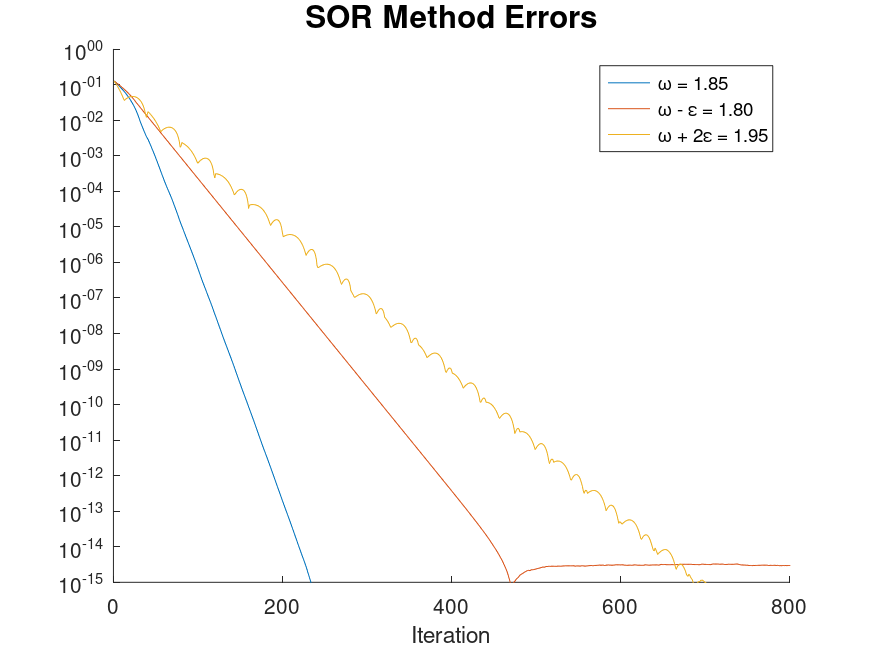
\includegraphics[width=0.7\textwidth]{problem_1b_sor_matrix_splitting_error_800_iterations.png}
        \caption{Iteration error for $\omega$ subject to perturbation}
    \end{figure}
\end{solution}